\documentclass[12pt,letterpaper]{standalone}
\usepackage{pgf, tikz}
\usepackage{mwe} % For dummy images 
\usetikzlibrary{positioning}
\usepackage{ifthen}
\usetikzlibrary{matrix,arrows.meta,quotes,shadows,decorations.pathreplacing,positioning,fadings}
\usepackage{cfr-lm}

\begin{document}
	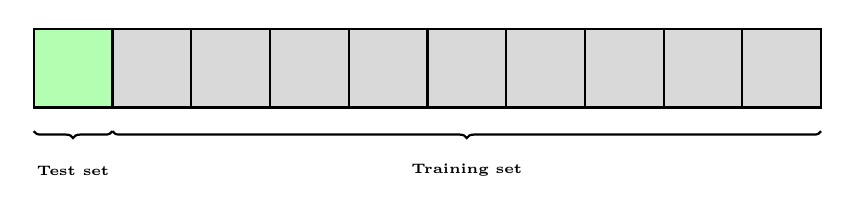
\begin{tikzpicture}
		\foreach \m in {0,...,9}
			\draw[thick, fill=gray!30] (\m,0) rectangle (\m+1, 1);
		\draw[thick, fill=green!30] (0,0) rectangle (1,1);
		
			\draw [
		thick,
		decoration={
			brace,
			mirror,
			raise=0.5cm
		},
		decorate
		] (0, 0.2) -- (1, 0.2);
		
		\node () at (0.5, -0.8) {\tiny \textbf{Test set}};
		
			\draw [
		thick,
		decoration={
			brace,
			mirror,
			raise=0.5cm
		},
		decorate
		] (1, 0.2) -- (10, 0.2);
		
		\node () at (5.5, -.8) {\tiny \textbf{Training set}};
	\end{tikzpicture}
\end{document}